\section{Databehandling}
\subsection{Afbildning med én samlelinse}
I dette forsøg, ændres positionen for linsen hvorefter skærmens position ændres, så billedet igen står skarpt. Der ønskes altså at undersøge sammenhængen mellem \cref{eq:fokalvokal}. Afstanden skiftes, mens $s$ og $s'$ bestemmes, så billedet står skarpt igen på skærmen.
Sammenhængen mellem $s$ og $s'$ for brændepunktet $f$ kan ses på \cref{fig:res1}.
\begin{figure}[H]
    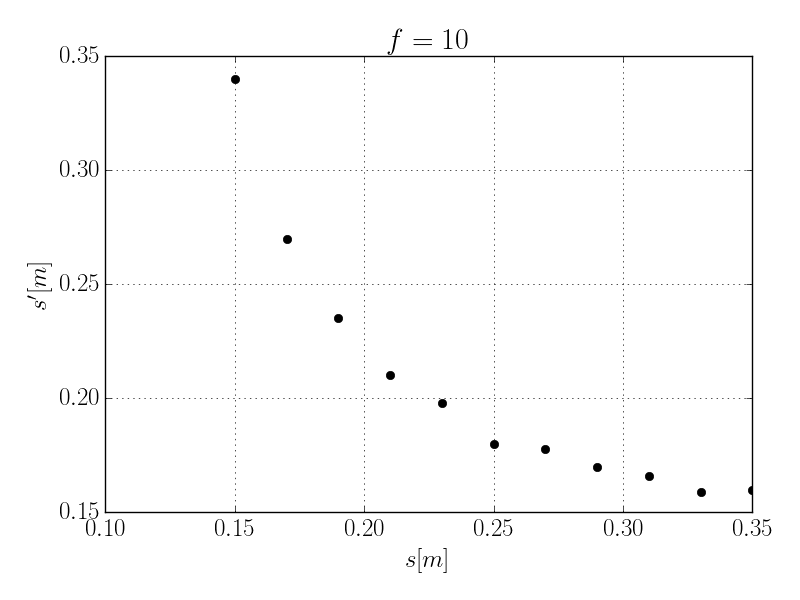
\includegraphics[width=\linewidth]{res1.png}
    \caption{Resultater af forsøg 1.}
    \label{fig:res1}
\end{figure}
Ved \cref{fig:res1} er forsøget angivet for datasæt1, hvor $f = 10$. Eksperimentet gentages desuden for datasæt2 hvor $f = 10$. Kun 4 Datapunkter, da vi ellers vil overskride lysbænkens længde.
\begin{figure}[H]
    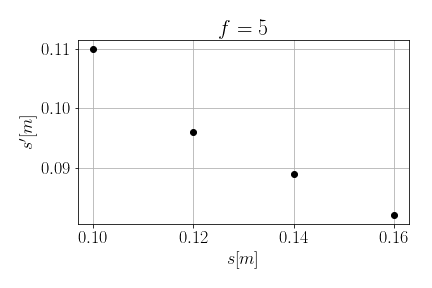
\includegraphics[width=\linewidth]{res2.png}
    \caption{Resultater af forsøg 2.}
    \label{fig:res2}
\end{figure}
Da fokuspunktet blev vurderet på øjemål, var det vores vurdering at det ikke kunne bestemmes til en sikkerhed på mindre end $\pm $ \SI{1}{\centi\meter}. På \cref{fig:usikkerhed} ses målingerne med usikkerheden.
\begin{figure}[H]
    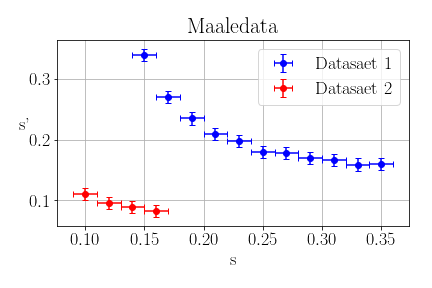
\includegraphics[width=\linewidth]{usikkerhed.png}
    \caption{Usikkerhed for målinger}
    \label{fig:usikkerhed}
\end{figure}
Der ses nu på datasæt 1. For at bestemme brændvidden for linsen plottes $\frac{1}{s'}$ som funktion af $\frac{1}{s}$. Da kan vi lave et fit med en ret linje, hvis skæring med 2. aksen vil netop være  $\frac{1}{f}$. Dette kan ses på \cref{fig:1}. Samme gentages for Datasæt 2 på \cref{fig:2}.
\begin{figure}[H]
    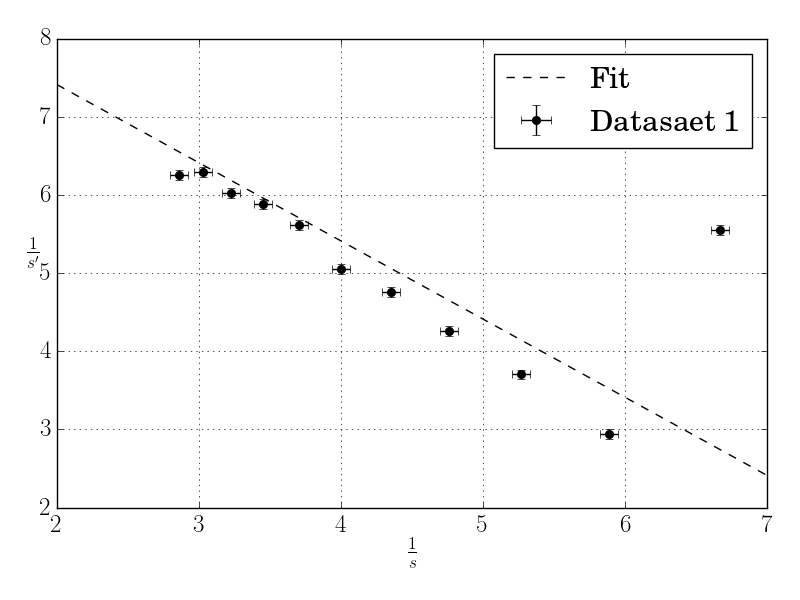
\includegraphics[width=\linewidth]{1.png}
    \caption{}
    \label{fig:1}
\end{figure}
\begin{figure}[H]
    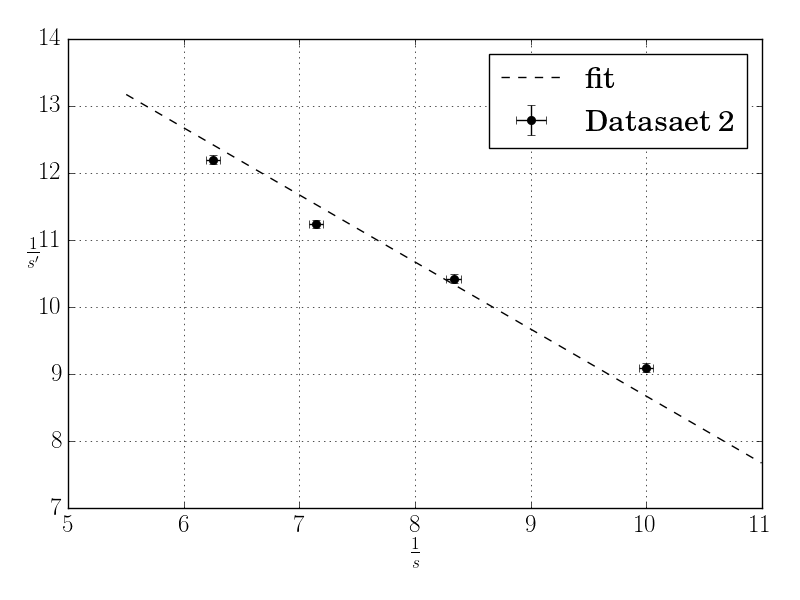
\includegraphics[width=\linewidth]{2.png}
    \caption{}
    \label{fig:2}
\end{figure}

Da findes fokallængderne ekserimentiel til at være for datasæt 1 og 2 til at være
\begin{align}
    \nonumber f_{10} &=  10,6 \pm \SI{3,5}{\centi\meter} \\
    \nonumber f_{5} &= 5,4 \pm \SI{3,9}{\centi\meter}
\end{align}
hvor usikkerhederne er bestemt vha. ophobningsloven.
\\ Ser vi på \cref{eq:m}, så ses det at man kan plotte $\frac{y'}{y}$ som funktion af $-\frac{s'}{s}$. Hvis data understøtter dette kan man tegne en ret linje med hældning 1 som burde skære datapunkterne perfekt. Dette ses på \cref{fig:3}.
\begin{figure}[H]
    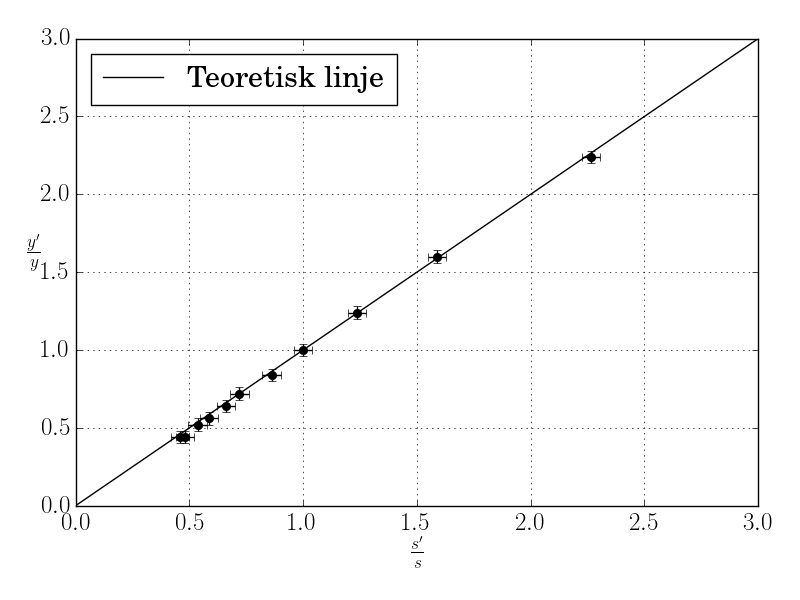
\includegraphics[width=\linewidth]{3.png}
    \caption{}
    \label{fig:3}
\end{figure}
Det ses på \cref{fig:3} at linjen ligger godt på datapunkterne, måske med en lille fejl ved de lavere værdier.
